\fe{\subsection{Exercices}}{\subsection{Exercises}}
\label{thermique_exo}

{\setbeamerfont{framesubtitle}{size=\tiny}
\begin{frame}{\fe{Exercice 3 : source dépendante de la température}
                 {Exercise 3: temperature-dependent heat source}}
             {\url{https://www-cast3m.cea.fr/index.php?page=exemples&exemple=formation_pasapas_3_initial}}
  \small
  \begin{itemize}
    \item \fe{Substrat chauffé par une source, refroidis par convection}
             {Substrate heated by a source, both are cooled by convection}\\
    \tiny
    \hspace{-0.5cm}
    \begin{tikzpicture}
      \node[anchor=south west,inner sep=0] (image) at (0,0)
      {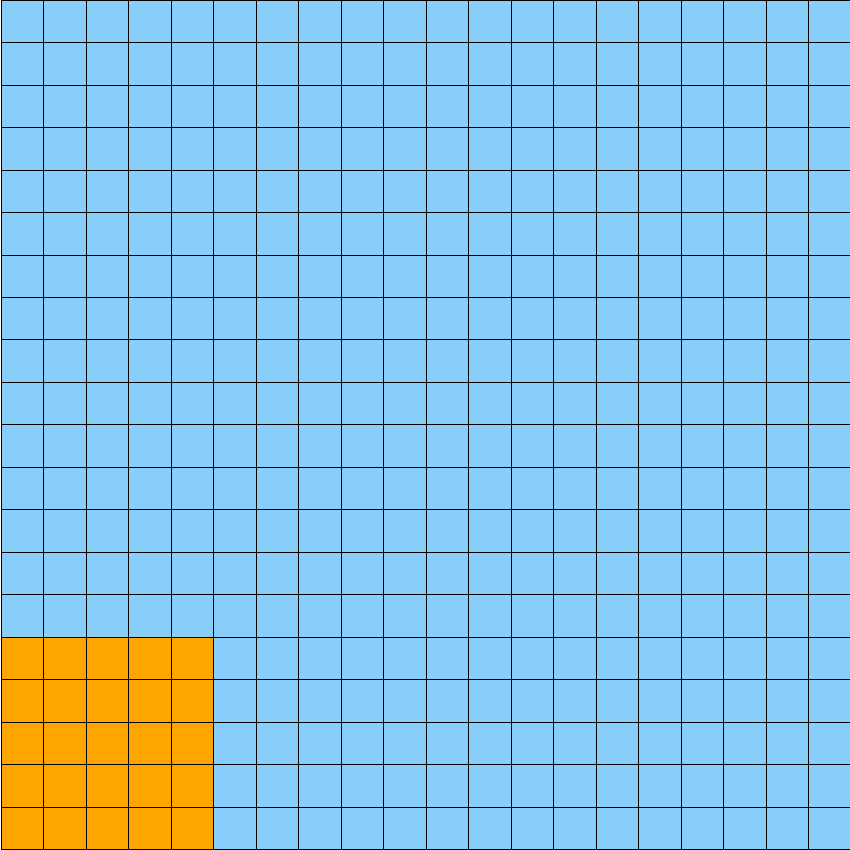
\includegraphics[height=1.8cm]{images/exo/exo_3_maillage}};
      \begin{scope}[x={(image.south east)},y={(image.north west)}]
        \draw[latex-latex,->] (0.2,1.) -- (0.5,0.55);
        \draw (0,1.2) node[anchor=north west]{Source $P_0=V.q_0$~=~1~W};
      \end{scope}
    \end{tikzpicture}
    \hspace{0.05cm}
    \if \animation 1
      \animategraphics[controls,loop,poster=last,height=3cm]{7}{images/exo/exo_3_temperature.}{01}{61}
    \else
      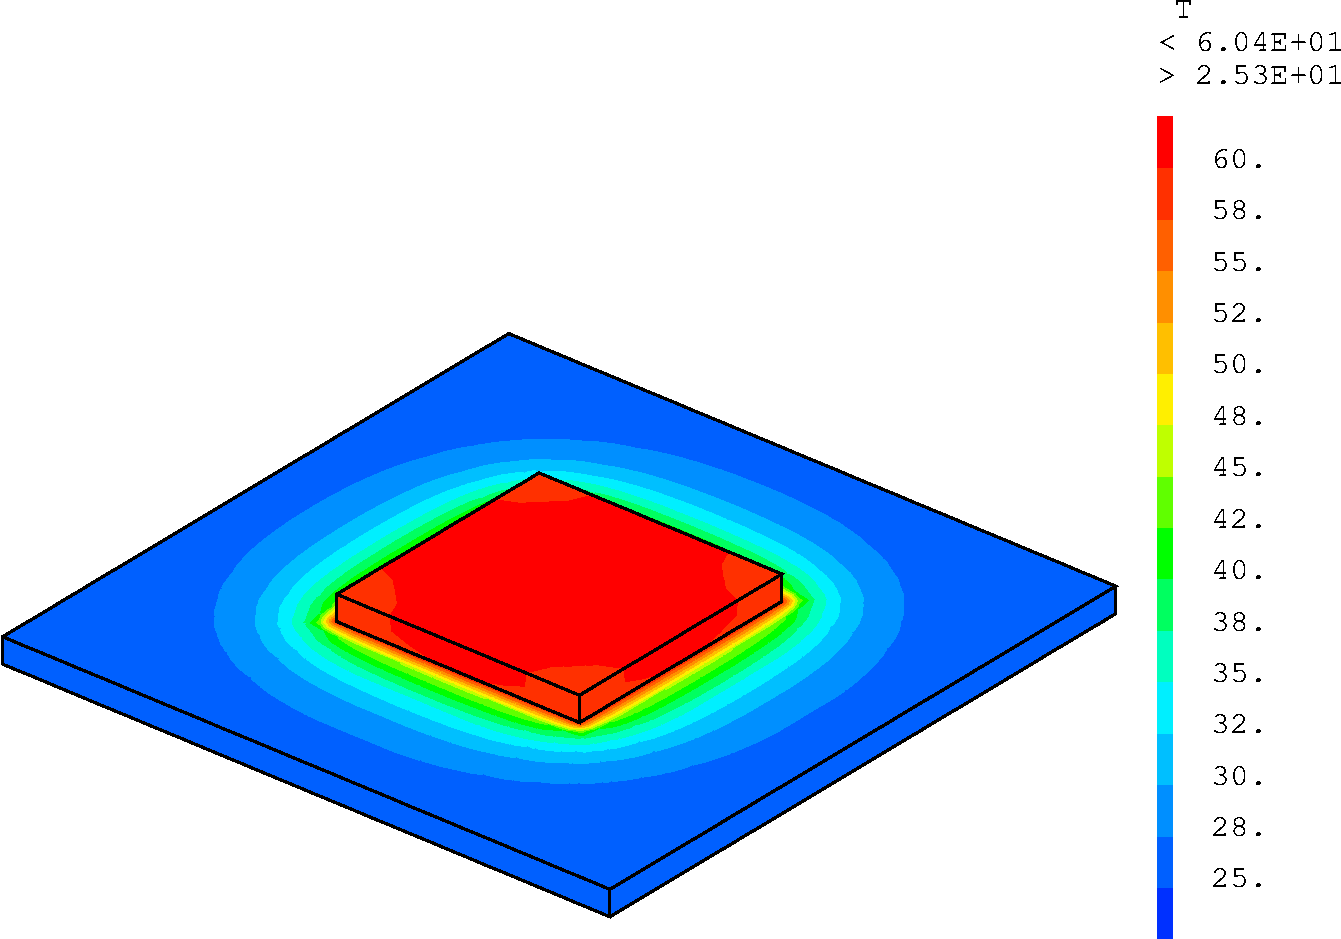
\includegraphics[height=3cm]{images/exo/exo_3_temperature.61}
    \fi
    \hspace{0.05cm}
    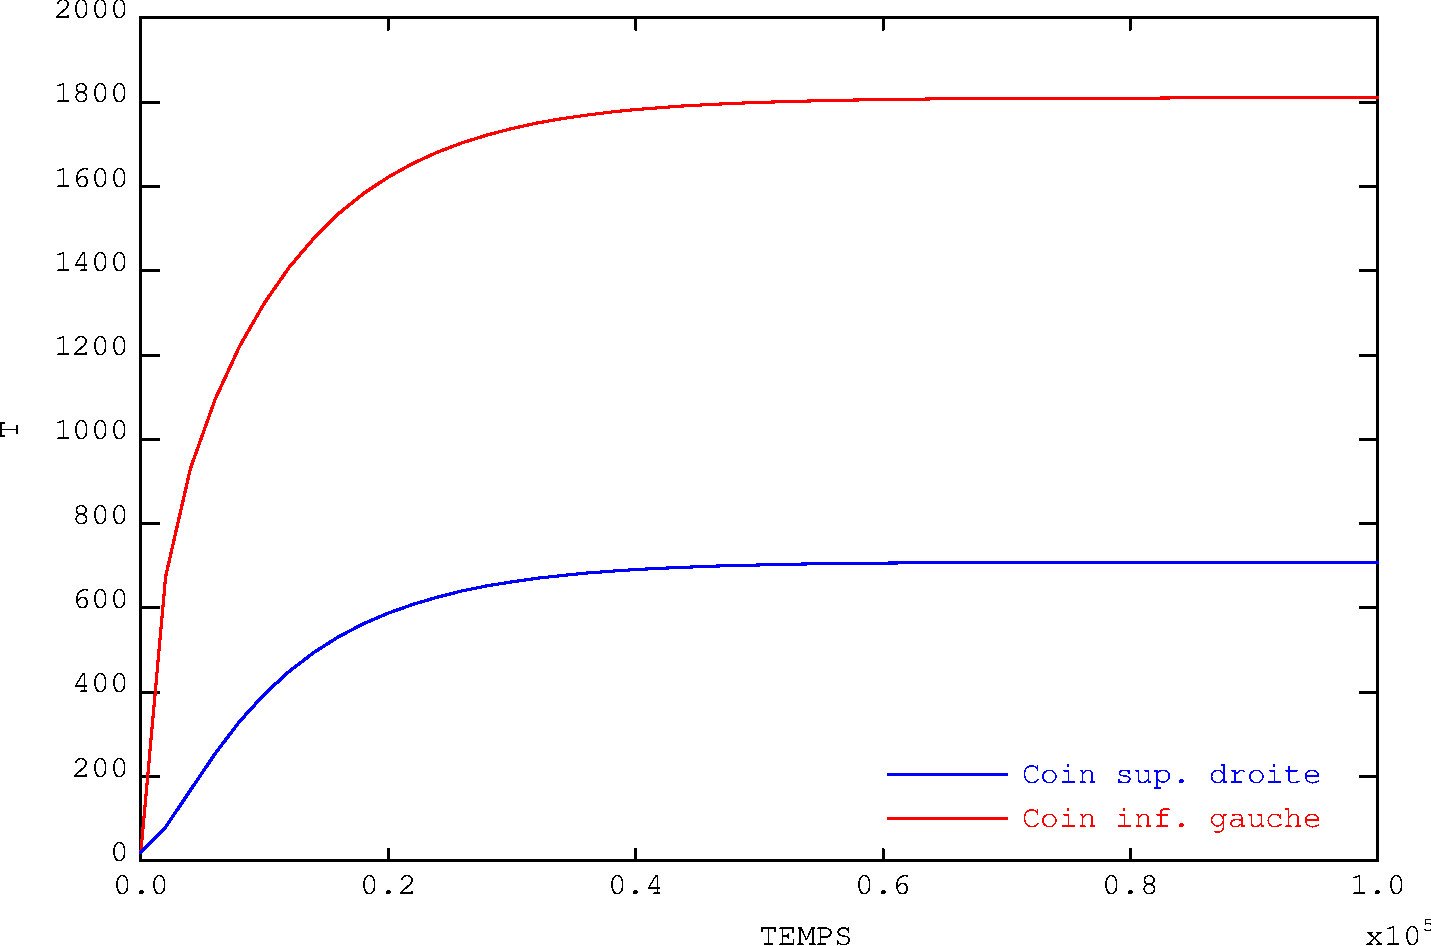
\includegraphics[height=2.5cm]{images/exo/exo_3_evol}
    \small
    \item<2-> \fe{\green{Objectif : modéliser une source \g{dépendante de la température}}}
                 {\green{Purpose: model a \g{temperature-dependent} heat source}}\\
    \fe{Loi d'Arrhenius:}{Arrhenius law:}
    $q(T)=q_0\dfrac{e^{-\frac{E_a}{k_b(T+273)}}}{e^{-\frac{E_a}{k_b(T_0+273)}}}$\\
    \scriptsize
    ~\\
    $E_a=0.15$~eV \qquad \fe{$k_b$ constante de Boltzmann}{$k_b$ Boltzmann constant}
    \begin{textblock*}{6cm}(8cm,-1.5cm)
      \begin{tikzpicture}
        \node[anchor=south west,inner sep=0] (image) at (0,0)
        {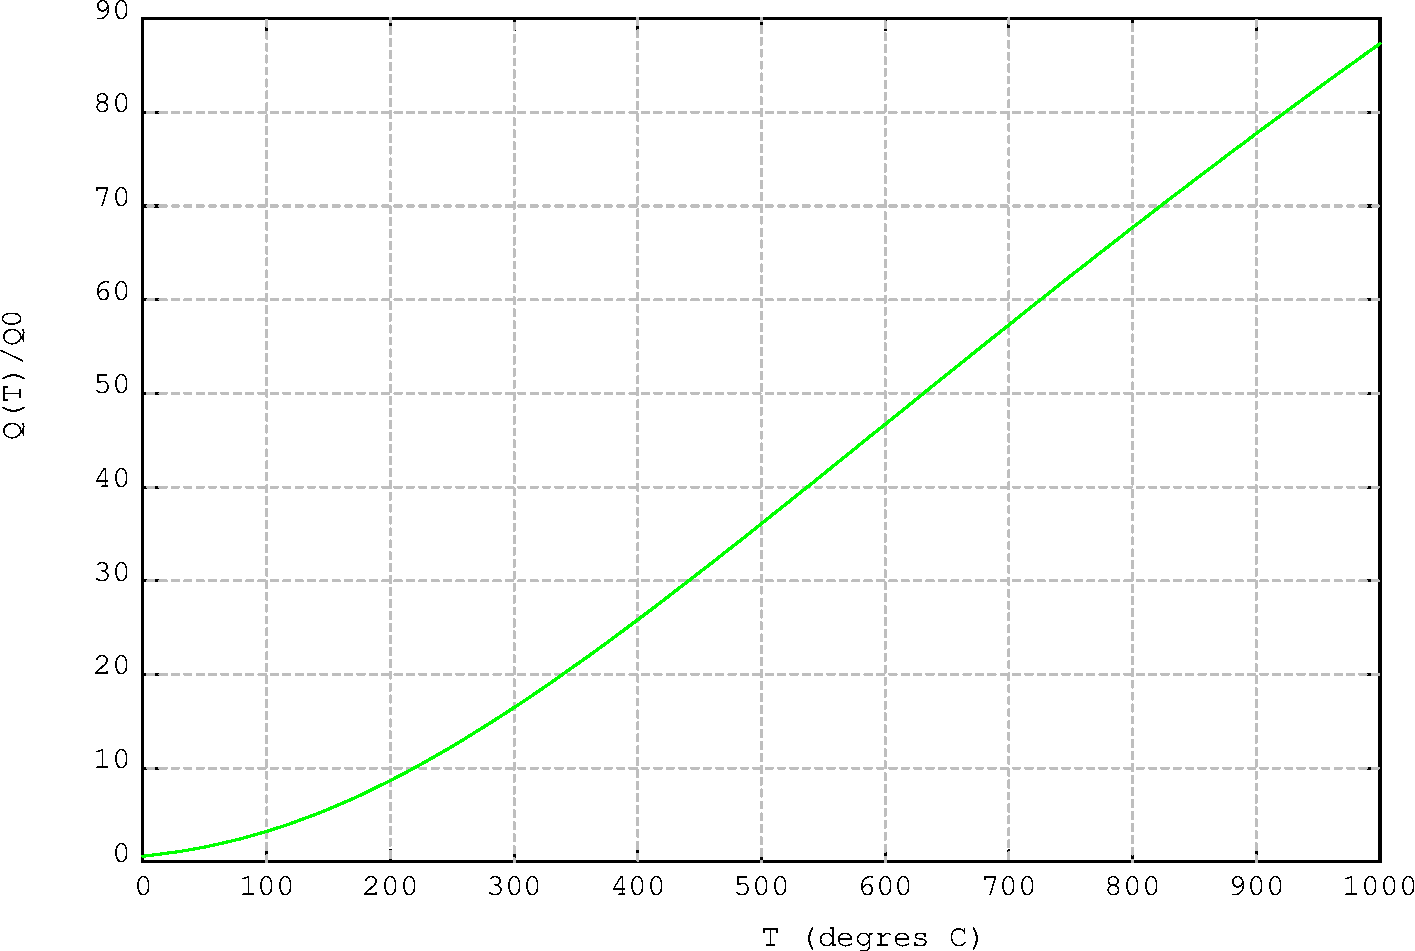
\includegraphics[height=2.7cm]{images/exo/exo_3_arrhenius}};
      \end{tikzpicture}
    \end{textblock*}
    \small
    \begin{center}
      \fe{\avous{~À vous de jouer !}}{\avous{~It's up to you!}}
    \end{center}
  \end{itemize}
\end{frame}
}

{\setbeamerfont{framesubtitle}{size=\tiny}
\begin{frame}{\fe{Exercice 3 : source dépendante de la température}
                 {Exercise 3: temperature-dependent heat source}}
             {\url{https://www-cast3m.cea.fr/index.php?page=exemples&exemple=formation_pasapas_3_initial}}
  \begin{itemize}
    \item \fe{Quelques objets utiles}{Some useful objects}\\
    \footnotesize
    \begin{tabular}{ll}
      \kw{sou, mosou} & \fe{maillage et modèle de la source de chaleur}{heat source mesh and model}\\
      \kw{q0}         & \fe{source volumique de chaleur à 25~°C}{volumetric heat source at 25~°C}
    \end{tabular}
    \normalsize
    \item \fe{Quelques opérateurs utiles}{Some useful operators}\\
    \footnotesize
    \begin{tabular}{ll}
      \kwr{REDU} & \fe{pour réduire les températures sur \kw{sou}}{to reduce temperatures on \kw{sou}}\\
      \kwr{IPOL} & \fe{pour interpoler la source volumique $q(T)$ selon le champ $T$}
                      {to interpolate the heat density $q(T)$ with $T$}\\
      \kwr{SOUR} & \fe{pour imposer une source volumique de chaleur}{to impose a volumetric heat source}
    \end{tabular}
    \normalsize
    \item \fe{Quelques indices utiles de la table}{Some useful table indices}\\
    \footnotesize
    \begin{tabular}{ll}
      \kwg{WTABLE}\kw{.}\kwg{THER\_COURANT} & \fe{températures courantes (itérations de \kwo{TRANSNON})}
                                                 {current temperatures (\kwo{TRANSNON} iterations)}
    \end{tabular}
    \normalsize
  \end{itemize}
\end{frame}
}

\begin{frame}{\fe{Exercice 3 : source dépendante de la température}
                 {Exercise 3: temperature-dependent heat source}}
             {\fe{Solution avec CHARTHER}{Solution with CHARTHER}}
  \footnotesize
  \begin{itemize}
    \small
    \item \fe{Définir une EVOLUTIOn pour $q(T)$}{Define an EVOLUTIOn for $q(T)$}
    \item \fe{Supprimer le CHARGEMEnt initial et utiliser \kwv{CHARTHER}}
             {Remove the initial load (CHARGEMEnt object) and use \kwv{CHARTHER}}
    \item \fe{Réduire le champ de température sur la source}{Reduce the temperature field on the source}
    \item \fe{Interpoler puis appliquer le champ de source}{Interpolate then apply the source field}
    \item[] ~
    \item[] ~
  \end{itemize}
  \vspace{4.5cm}
  \scriptsize
  \begin{textblock*}{10cm}(0.3cm,-5.2cm)
    \fe{\emph{Programme principal}}{\emph{Main program}}
    \lstinputlisting[basicstyle=\ttfamily\tiny, language=gibiane, firstline=72, lastline=77]{dgibi/formation_pasapas_3_solution.dgibi}
    \lstinputlisting[basicstyle=\ttfamily\tiny, language=gibiane, firstline=108, lastline=110]{dgibi/formation_pasapas_3_solution.dgibi}
  \end{textblock*}
  \begin{textblock*}{10cm}(6.cm,-2.8cm)
    \fe{\emph{\violet{Procédure CHARTHER}}}{\emph{\violet{CHARTHER procedure}}}
    \lstinputlisting[basicstyle=\ttfamily\tiny, language=gibiane, firstline=86, lastline=93]{dgibi/formation_pasapas_3_solution.dgibi}
  \end{textblock*}
\end{frame}

\begin{frame}{\fe{Exercice 3 : source dépendante de la température}
  {Exercise 3: temperature-dependent heat source}}
{\fe{Solution avec CHARTHER}{Solution with CHARTHER}}
\begin{itemize}
    \item \fe{Résultats}{Results}\\
    \if \animation 1
      \animategraphics[controls,loop,poster=last,width=5cm]{7}{images/exo/exo_3_solu_temperature.}{01}{61}
    \else
      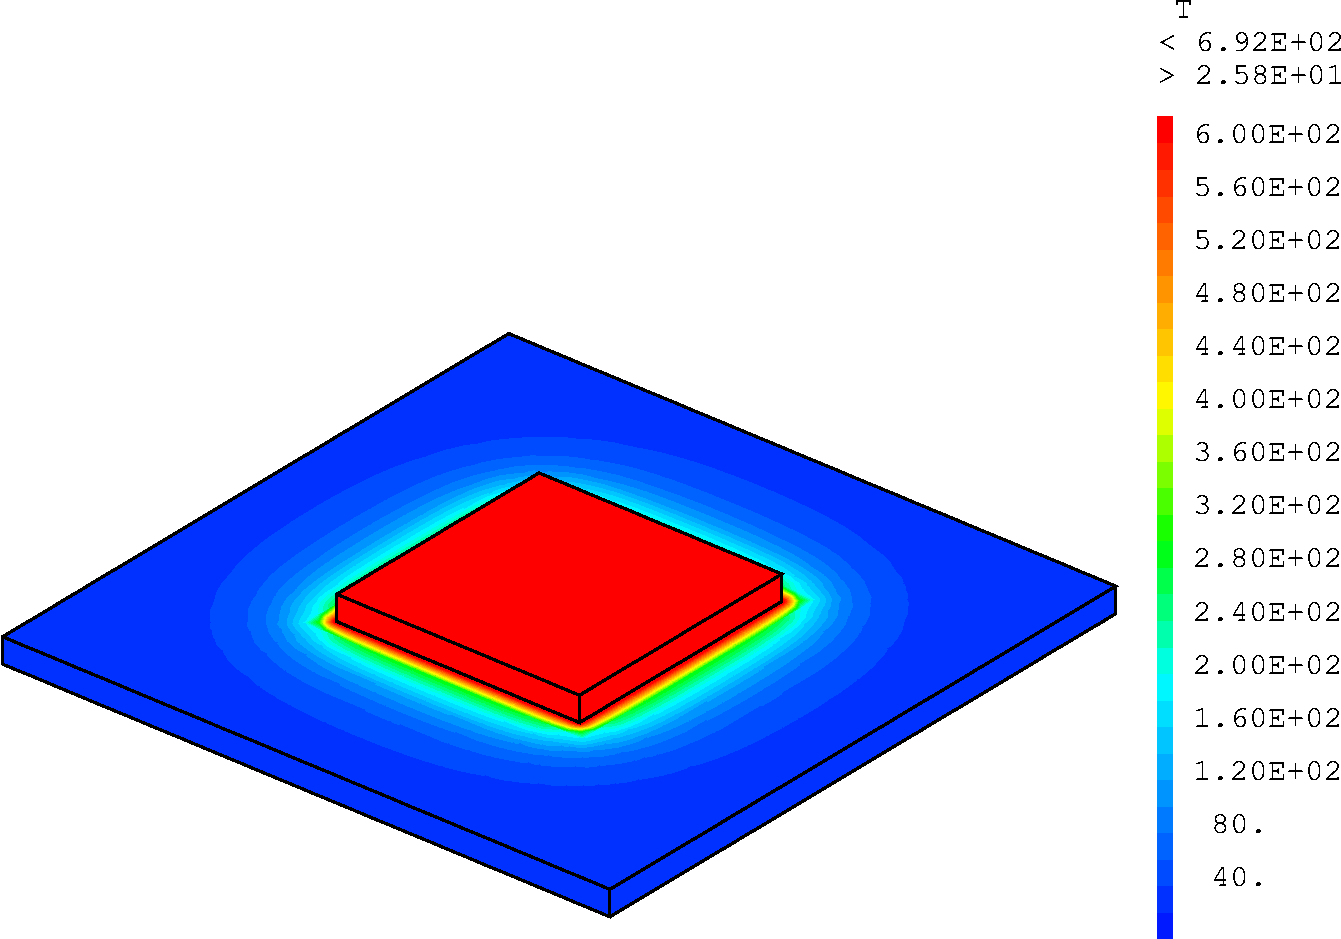
\includegraphics[width=5cm]{images/exo/exo_3_solu_temperature.61}
    \fi
    \hspace{0.5cm}
    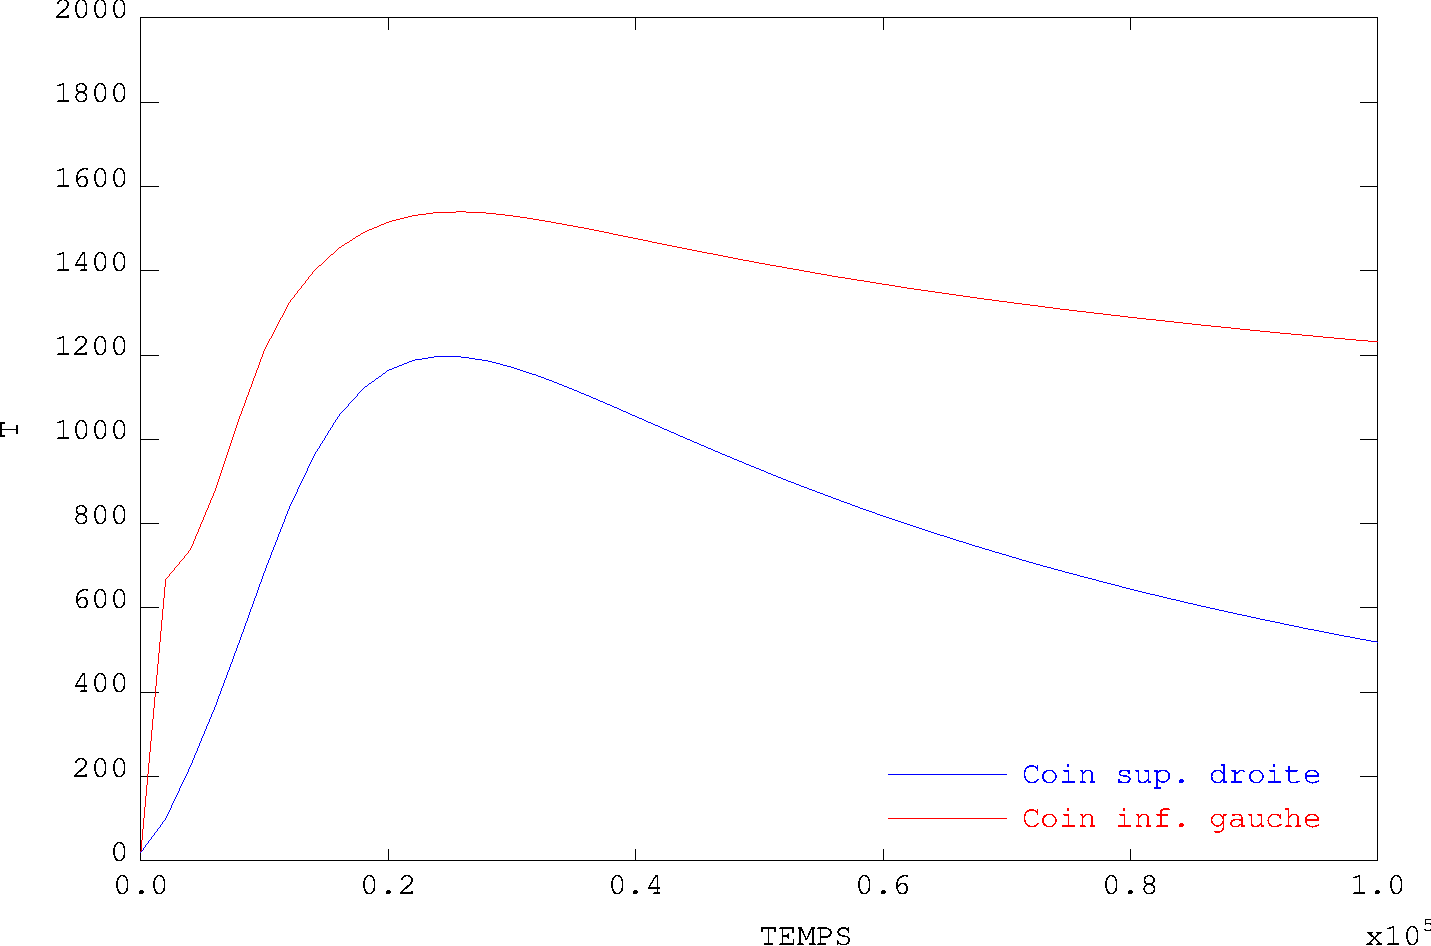
\includegraphics[width=5cm]{images/exo/exo_3_solu_evol}
  \end{itemize}
\end{frame}
